%% SIViP submission (Springer Nature sn-jnl, double-column)
%% Download the official template: https://www.springernature.com/gp/authors/campaigns/latex-authoring
%% Place sn-jnl.cls and required .bst in this folder. Compile with pdflatex + bibtex.
\documentclass[sn-mathphys-num,iicol]{sn-jnl}

\usepackage{graphicx}
\usepackage{amsmath,amssymb,amsfonts}
\usepackage{booktabs}
\usepackage{array}
\usepackage{multirow}
\usepackage{siunitx}
\usepackage{tikz}
\usetikzlibrary{arrows.meta,positioning}

\raggedbottom

\begin{document}

\hypersetup{%
  pdftitle={Background-Input Leakage in Video Foreground Segmentation: An Empirical Audit and a Frozen Causal Protocol},
  pdfauthor={Jichao Liu},
  pdfkeywords={video foreground segmentation, background subtraction, background-input leakage, self-distillation, evaluation protocol, reproducibility}}

\title[Background-Input Leakage in Video Foreground Segmentation]{%
Background-Input Leakage in Video Foreground Segmentation: An Empirical Audit and a Frozen Causal Protocol}

\author*[1]{\fnm{Jichao} \sur{Liu}}\email{liujichao09@haier.com}
\affil*[1]{\orgname{Hainayun IoT Technology Co., Ltd.}, \orgaddress{\city{Qingdao}, \state{Shandong}, \postcode{266103}, \country{China}}; ORCID: 0000-0001-5767-8654}

\abstract{%
Background-image guided networks are a popular paradigm for video foreground
segmentation: a background image, often produced by a background-subtraction
(BGS) algorithm such as SuBSENSE, is fed to a convolutional network together with
the current frame, and is often trained with the same BGS masks as pseudo-labels.
Its provenance---past frames, BGS-guided, or future-frame oracle---is rarely
reported, making numbers incomparable. This paper contributes an empirical audit and protocol, not a new
architecture. We formalize three leakage channels (background-input leakage,
pseudo-label self-distillation, and future-frame oracle), define
causal/leaky/oracle provenance levels, and introduce leakage-gap and oracle-gap
metrics. Holding weights fixed and switching only the background source for a
reproduced GNet on four held-out categories, the domain model drops from
F1 = 0.6661 (leaky) to 0.4526 (causal), a relative drop of 32\%, and remains
below its SuBSENSE teacher (0.7256). The oracle gap is +0.159 for the domain
model but only +0.021 for the synthetic model. Under a frozen causal protocol (stride 1), the synthetic
background+CNN model (0.290 $\pm$ 0.041) does not outperform a non-learning
causal residual threshold (0.392) or SuBSENSE (0.729); the same holds on SBI 2015
(0.347 vs.\ 0.589). A label-free causal teacher raises a same-domain model to
0.417, below its own teacher (0.465) and far below SuBSENSE;
reliability-gating, boundary and
degradation variants (0.240/0.249/0.260) show no consistent gain. Seed variance
(0.041) exceeds most ablation differences. We recommend reporting provenance,
teacher baselines, a frozen protocol and seed variance, and separating method
gains from leakage. Code, video splits and per-video results are released.}

\keywords{video foreground segmentation, background subtraction,
background-input leakage, self-distillation, evaluation protocol, reproducibility}

\maketitle

\section{Introduction}\label{sec:intro}

Video foreground segmentation is a fundamental component of video surveillance,
traffic monitoring and scene understanding. The CDnet 2014 benchmark
\cite{cdnet2014} has made the task reproducible at the dataset level, and
background subtraction (BGS) remains a strong and inexpensive baseline
\cite{stauffer1999,vibe2011,subsense2015,pbas2012}.
In recent years, a popular paradigm has emerged: a background image, usually
produced by a BGS algorithm such as SuBSENSE \cite{subsense2015}, is fed to a
convolutional network together with the current frame, and the network predicts
a foreground mask. Representative methods include background-model-image
networks \cite{kimbgsub2020}, scene-specific and video-agnostic supervised models
\cite{braham2016,babaee2018,fgsegnet2018,fgsegnetv2_2020,bsuvnet2020,bsuvnet2021,bgsubnet2024},
and zero-shot background modeling \cite{zbs2023}. The paradigm is intuitive:
the background provides a pixel-aligned reference, and the network learns where
the current frame deviates from it.

The difficulty is that the reported accuracy of this paradigm conflates three
sources of gain. First, the background input itself may contain the test-time
BGS decision. If the background is updated only on pixels that SuBSENSE classifies
as background, then the residual between the current frame and the background
already approximates the SuBSENSE mask, so a network can reproduce the BGS
decision without learning transferable foreground cues. Second, if the training
labels are also generated by the same BGS, the network is distilled from its
teacher; its domain-specific gain may then reflect self-distillation rather than
a new mechanism. Third, if the background is estimated from the whole test
sequence, for example as the temporal median of all frames or as the static
background distributed with a dataset, the evaluation uses future frames and
therefore constitutes an oracle. We refer to these three phenomena as
background-input leakage, pseudo-label self-distillation, and future-frame
oracle, respectively.

These channels are not exotic corner cases. They are common consequences of
standard engineering choices: BGS-guided background updates are natural when a
BGS mask is available, pseudo-labels are natural when manual annotation is
expensive, and whole-video medians are natural when a static background is
available. What is often missing is the provenance of the background in the
reported result. Without provenance, a number such as ``F1 = 0.96'' cannot be
compared with a number obtained under a causal protocol, because the two numbers
may measure different quantities. This is the problem we address.

We do not propose a new segmentation network. Instead, we treat a reproduced
GNet as a controlled testbed and ask what happens when only the background
source changes. We define three provenance levels---causal, leaky and
oracle---and two descriptive metrics: the leakage gap $\Delta_{\mathrm{leak}}$
and the oracle gap $\Delta_{\mathrm{oracle}}$. The former quantifies how much
performance is available through BGS-guided background updates; the latter
quantifies how much performance is available through future frames. We then
measure both gaps with fixed weights, fixed frames and fixed post-processing, so
that the only variable is the background estimator. We complement this
controlled comparison with a strict-causal evaluation against non-learning
baselines, a multi-seed variance analysis, a cross-dataset check on SBI 2015,
and a released reproducibility package.

Our contributions are audit-oriented:
\begin{enumerate}
\item We formalize three leakage channels in background-guided video foreground
segmentation and define causal/leaky/oracle provenance levels together with
leakage-gap and oracle-gap metrics (Section~\ref{sec:protocol}).
\item We perform a same-weight, provenance-only switching experiment and
quantify the dependence of a domain-trained model on BGS-guided backgrounds
($-0.214$ F1) and on future-frame backgrounds ($+0.160$) (Section~\ref{sec:rq1}).
\item We report a strict-causal negative result: a synthetic
background+CNN pipeline ($0.290\pm0.041$) does not outperform a non-learning
causal residual threshold ($0.392$) or SuBSENSE ($0.729$), and the same
qualitative conclusion holds on SBI 2015 (Section~\ref{sec:rq3},
Section~\ref{sec:rq5}). A label-free causal teacher yields 0.417 on the same
four held-out categories, below the SuBSENSE teacher (0.726), and reliability,
boundary and degradation variants do not improve on the synthetic baseline
(Section~\ref{sec:rq3}, Section~\ref{sec:rq6}).
\item We show that seed variance ($0.041$) exceeds most ablation differences and
that a reliability-gating variant does not consistently improve accuracy, and we distill these
findings into a reporting checklist, and we release the code, splits and
per-video results (Section~\ref{sec:rq4}, Section~\ref{sec:rq6},
Section~\ref{sec:disc}).
\end{enumerate}

We are explicit about what we do not claim. We do not claim state-of-the-art accuracy, we
do not claim that our testbed covers all architectures or background estimators,
and we do not claim that every background-guided method leaks to the same
degree. Our claims concern the provenance levels we can control and the
models we can reproduce. The broader message is methodological: because
provenance can change F1 by more than twenty points, it must be reported.

\section{Related Work}\label{sec:related}

\subsection{Background-guided foreground segmentation}
Background-model-image networks concatenate or fuse a background image with the
current frame. Representative examples include Kim and Ha \cite{kimbgsub2020},
scene-specific CNNs \cite{braham2016,babaee2018}, BSUV-Net \cite{bsuvnet2020}
and BSUV-Net 2.0 \cite{bsuvnet2021}, and BgSubNet \cite{bgsubnet2024}.
Table~\ref{tab:litprov} summarizes the provenance of representative methods: it
ranges from BGS-generated and manually selected backgrounds to offline
whole-video reconstruction and synthetic/paired backgrounds; two further
methods (Braham \cite{braham2016}; Babaee \cite{babaee2018}) do not state the source in the accessible materials.
Provenance is therefore often implicit, and in several cases it is not stated at all.
BgSubNet uses synthetic pretraining and semi-supervised fine-tuning, but the
real-scene background source is not stated in the accessible abstract.
By contrast, FgSegNet and FgSegNet v2 \cite{fgsegnet2018,fgsegnetv2_2020}, ZBS
\cite{zbs2023}, motion-based video object segmentation
\cite{motionasoption2025}, and BGS-only methods \cite{sttrpca2025,ganbgs2025} do
not take a background image. Our claims therefore concern the background-image
subset, not all video foreground segmentation; the design question is where the
background comes from, and whether that source uses BGS decisions or future
frames. The released audit file extends Table~\ref{tab:litprov} to 14 methods,
including frame-only, zero-shot, motion-based and BGS-only methods.

\begin{table*}[t]
\centering
\scriptsize
\setlength{\tabcolsep}{3pt}
\caption{Background provenance of representative background-image methods.
n.s.: not stated; BGS: background generated/updated by a BGS algorithm; manual:
empty background selected from the test video; offline: uses the complete
video; Code: public code/weights found (n.s. = not found/verified).}
\label{tab:litprov}
\begin{tabular}{@{}>{\raggedright\arraybackslash}p{24mm}>{\raggedright\arraybackslash}p{28mm}>{\raggedright\arraybackslash}p{57mm}>{\raggedright\arraybackslash}p{13mm}>{\raggedright\arraybackslash}p{8mm}@{}}
\toprule
Method & Input & Background source & Online & Code \\
\midrule
Kim \cite{kimbgsub2020} & BG + frames & SuBSENSE-gen. & BGS & n.s. \\
BSUV-Net \cite{bsuvnet2020} & frame + 2 BG + FPM & empty: selected median; recent: 100-frame median & manual + causal & yes \\
BSUV-Net 2.0 \cite{bsuvnet2021} & frame + 2 BG + FPM & manual empty + 100-frame median & manual + causal & yes \\
BgSubNet \cite{bgsubnet2024} & image + BG & BG image (source n.s.) & n.s. & n.s. \\
Autoencoder \cite{autonoise2023} & frame + recon. BG & complete-video AE + median & offline & n.s. \\
\bottomrule
\end{tabular}
\end{table*}

\subsection{Unsupervised and self-supervised BGS}
Unsupervised BGS ranges from Gaussian mixture and non-parametric models
\cite{stauffer1999,elgammal2000,gmmreview2017} to sample-based and self-organizing
methods \cite{vibe2011,sobs2008,pbas2012,subsense2015}; see
\cite{bouwmans2014,garcia2020,sobral2014} for surveys. Recent examples include
generator-discriminator learning \cite{ganbgs2025} and tensor RPCA
\cite{sttrpca2025}. These methods are usually evaluated as standalone BGS. When
their output becomes a network input, the provenance question reappears: the
network may exploit the estimator's decision, and the gain may not transfer. Our
switching experiment exposes this dependence.

\subsection{Input cues, shortcuts and over-reliance}
The idea that a network can over-rely on a cue that is correlated with the label
is well established. Shortcut learning \cite{shortcut2020} and the Clever Hans
phenomenon \cite{cleverhans2019} show that classifiers can exploit incidental
correlations that do not transfer. In data mining and machine learning more
broadly, the same failure mode is studied as leakage
\cite{leakage2012,leakage2023}. Motion-as-Option
\cite{motionasoption2025} shows that optical flow is strongly correlated with
foreground masks and that networks can over-depend on motion, becoming unstable
under confusing motion. We study the same phenomenon for a different cue: the
background input. In the leaky setting, the background is correlated with the BGS
mask, and a network can exploit this correlation. The leakage gap is an
operational measure of how much of the reported performance is consistent with
such exploitation. Pseudo-label self-distillation is the related channel: a student can fit its
teacher's errors \cite{noisystudent2020,confirmationbias2020}, so the teacher
baseline is needed.

\subsection{Background noise and uncertainty}
Several works estimate the reliability of a reconstructed background. An
autoencoder-based method predicts background noise for thresholding
\cite{autonoise2023}, and uncertainty estimation for deep networks is surveyed in
\cite{uncertainty2023}. These works motivate per-pixel reliability, but
reliability is not the focus of our audit. We include a reliability-gated variant
as a diagnostic and report a negative result: the variant does not improve
accuracy under our protocol. This negative result is useful because it separates
``the background is unreliable'' from ``a learned reliability gate improves
segmentation''; the two claims are often conflated.

\subsection{Evaluation protocols and reproducibility}
CDnet 2014 \cite{cdnet2014}, its earlier version \cite{cdnet2012}, and SBI 2015
\cite{sbi2015,sbitax2017} are widely used, but protocol details such as frame
stride, shadow handling, region-of-interest masking and aggregation can change
reported numbers; see \cite{sobral2014} for an evaluation study. Segmentation
measures themselves are not interchangeable, as discussed for boundary and
region metrics in \cite{evalmeasure2013}. Reproducibility is further complicated when code, weights, splits or background
estimators are unavailable \cite{leakage2023}, and seed variance is routinely
under-reported \cite{drlmatters2018,scoredist2017,showyourwork2019}. Our
protocol fixes these choices and reports them explicitly.

\subsection{Video object segmentation benchmarks}
Semi-supervised video object segmentation methods such as OSVOS
\cite{osvos2017} and the DAVIS benchmark \cite{davis2016} also produce per-frame
foreground masks, but they assume a first-frame annotation and are evaluated with
region and boundary measures designed for that setting. Our task is unsupervised
background subtraction without a first-frame mask, so these methods are not
direct baselines; we cite them only to delimit the scope of the audit.

\section{Audit Design and Protocol}\label{sec:protocol}

\subsection{Background provenance levels}\label{sec:provenance}

Let $I_{1:T}$ be a video and let $B_t$ be the background used at time $t$. We
distinguish three provenance levels; Figure~\ref{fig:provenance} summarizes the
controlled switching design and the channels attached to each level.
\begin{itemize}
\item \textbf{Causal.} $B_t = f(I_{1:t})$ with $f$ using only current and past
frames, and using neither segmentation labels nor BGS masks. A running average or
a causal temporal median are examples.
\item \textbf{Leaky.} $B_t = f(I_{1:t}, M_{1:t}^{\mathrm{BGS}})$, where
$M^{\mathrm{BGS}}$ is a BGS mask. A typical example updates the background only
on pixels classified as background. The background is still causal in time, but
it carries the BGS decision.
\item \textbf{Oracle.} $B_t = f(I_{1:T})$ uses future frames. The temporal median
of the whole video and the static background distributed with a dataset are
examples.
\end{itemize}

The term ``leaky'' is operational. Using a BGS output is not by itself an error:
if the goal is to post-process a BGS result, a BGS-guided background is a
legitimate design. The problem arises when a method claims to learn transferable
foreground cues or cross-scene generalization while its background input carries
the test-time BGS decision. In that case the reported gain and the claimed
mechanism refer to different things.

\subsection{Leakage channels}\label{sec:leakage}

We distinguish three channels.
\begin{description}
\item[L1: background-input leakage.] The background input encodes the BGS
decision. A network can reproduce the decision from the input without learning
foreground appearance.
\item[L2: pseudo-label self-distillation.] The training labels and the inference
background come from the same BGS. The model is then distilled from its teacher,
and its gain should be compared with the teacher's accuracy.
\item[L3: future-frame oracle.] The background uses frames after $t$. The
evaluation measures a quantity that is unavailable online.
\end{description}

The channels can co-occur. A domain-trained model that is trained with SuBSENSE
pseudo-labels and evaluated with a SuBSENSE-guided running background is exposed
to L1 and L2 simultaneously. An evaluation that uses a whole-video median is
exposed to L3. Our experiments are designed to separate L1/L3 from L2 where
possible: in the provenance-switching experiment the weights are fixed, so any
change is due to the input channel; in the self-distillation test we compare the
model with its teacher.

\subsection{Gap metrics}\label{sec:metrics}

For a fixed model and test set, we define
\begin{equation}
\begin{aligned}
\Delta_{\mathrm{leak}} &= \mathrm{F1}_{\mathrm{leaky}} -
\mathrm{F1}_{\mathrm{causal}},\\
\Delta_{\mathrm{oracle}} &= \mathrm{F1}_{\mathrm{oracle}} -
\mathrm{F1}_{\mathrm{causal}}.
\end{aligned}
\label{eq:gaps}
\end{equation}
A positive $\Delta_{\mathrm{leak}}$ indicates that performance increases when the
background input carries BGS decisions; a positive $\Delta_{\mathrm{oracle}}$
indicates that performance increases when future frames are available. Smaller
gaps are desirable for a method that claims online, leakage-free operation. We
emphasize that the gaps are descriptive: they quantify the exploitable dependence
under the tested background estimators, not a causal effect of leakage in
general. We report F1, percentage of wrong classifications (PWC) and boundary F1
(BF1), with F1 as the primary metric; BF1 follows the boundary-band evaluation
discussed in \cite{evalmeasure2013}. For the boundary metric we use a 2-pixel
tolerance band around the ground-truth contour.

\subsection{Frozen causal protocol}\label{sec:frozen}

All strict-causal results use the following protocol: all frames inside the
temporal region of interest, stride 1; shadows counted as background; pixels
outside the region of interest ignored; per-video F1 first, then the arithmetic
mean over categories; decision threshold 0.5. The same weights, frames and
post-processing are used across provenance levels; only the background estimator
changes. Non-learning residual baselines scan a threshold $\tau$ on the test set
and report the best category-average F1. This makes the non-learning baselines
optimistic, which is deliberate: it prevents us from overstating the difficulty
of the baseline. The controlled provenance-switching experiment in
Section~\ref{sec:rq1} uses the same stride-1 protocol on four held-out
categories. All provenance levels in that experiment use the same weights and
frames, so the only variable is the background source.

\subsection{Controlled testbed}\label{sec:testbed}

We reproduce a GNet-style network as a testbed: a ResNet101 dual encoder, an
ASPP module, and a temporal self-attention module (TSAM) with 12 layers and 8
heads, operating on $513\times513$ inputs. The network takes the current frame
and a background image and predicts a foreground mask at the same resolution.
The \emph{synthetic} model is trained on composited Cityscapes \cite{cityscapes2016}
and COCO \cite{coco2014} images; its background is a causal exponential moving
average. The \emph{domain} model is trained on seven CDnet categories and tested
on four held-out categories; it follows the original paradigm, using SuBSENSE
pseudo-labels and a SuBSENSE-guided background. The \emph{reliability} variant
adds a learned per-pixel gate on the feature difference; it is a diagnostic, not
the main object of study. We also consider a \emph{full} variant that adds
boundary attention and background-degradation simulation, and a \emph{label-free}
variant trained with a causal-median teacher. These variants are diagnostics: as
shown in Section~\ref{sec:rq3}, none of them improves on the synthetic baseline
under the strict protocol. The testbed is audited, not proposed as a new method.

\begin{figure}[t]
\centering
\resizebox{\linewidth}{!}{%
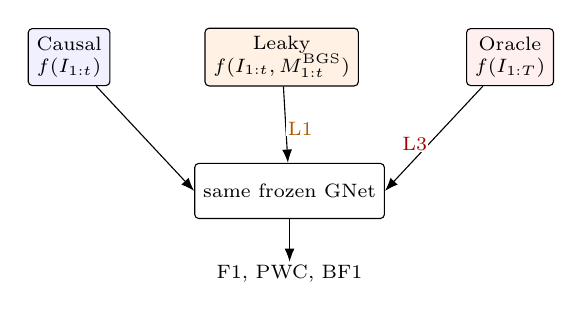
\begin{tikzpicture}[font=\scriptsize,>=Latex,
  box/.style={draw,rounded corners=1.5pt,align=center,inner sep=3pt,minimum height=7mm},
  lab/.style={align=center,inner sep=1pt}]
\node[box,fill=blue!6] (c) at (0,0) {Causal\\ $f(I_{1:t})$};
\node[box,fill=orange!10] (l) at (2.7,0) {Leaky\\ $f(I_{1:t},M^{\mathrm{BGS}}_{1:t})$};
\node[box,fill=red!6] (o) at (5.6,0) {Oracle\\ $f(I_{1:T})$};
\node[box] (g) at (2.8,-1.7) {same frozen GNet};
\node[lab] (f) at (2.8,-2.75) {F1, PWC, BF1};
\draw[->] (c) -- (g.west);
\draw[->] (l) -- node[right,orange!70!black,pos=0.55,fill=white,inner sep=0.5pt] {L1} (g);
\draw[->] (o) -- node[left,red!65!black,pos=0.55,fill=white,inner sep=0.5pt] {L3} (g.east);
\draw[->] (g) -- (f);
\end{tikzpicture}%
}
\caption{Background provenance and the three leakage channels. The audit holds
the network weights fixed and changes only the background estimator: leaky
backgrounds carry the BGS decision (L1), training labels may come from the same
BGS (L2), and oracle backgrounds use future frames (L3).}
\label{fig:provenance}
\end{figure}

\section{Experiments}\label{sec:exp}

\subsection{Datasets, splits and implementation}\label{sec:setup}

The main evaluation uses CDnet 2014 \cite{cdnet2014}: 53 videos in 11 categories.
The synthetic model is trained on Cityscapes and COCO composites and never sees a
CDnet video. The domain model uses a category-held-out split: it trains on seven
categories and tests on badWeather, nightVideos, turbulence and thermal, with no
video overlap. The cross-dataset evaluation uses SBI 2015 \cite{sbi2015,sbitax2017}; no model
is trained on SBI. Video-level split files and evaluation commands are released.

The network is trained with SGD at learning rate $0.01$, momentum $0.9$ and weight
decay $5\times10^{-4}$, with cosine annealing, for 8 epochs of 600 steps, batch
size 8. The seeds are $\{0,1,2\}$ for the synthetic model. The input size is
$513\times513$. All reported numbers are category averages on the corresponding
test sets.

\subsection{RQ1: Does background provenance change results at fixed weights?}\label{sec:rq1}

Table~\ref{tab:provenance} reports the same weights evaluated with four
background sources on the four held-out categories. The four sources are
\emph{leaky} (a causal running average updated only on SuBSENSE background
pixels), \emph{causal} (a mask-free causal running average), \emph{first frame}
(a static first frame), and \emph{oracle} (the static background distributed with
CDnet, which is essentially the whole-video temporal median; its mean absolute
difference from the whole-video median is 0.22/255).

\begin{table*}[t]
\centering
\small
\caption{Background-provenance switching at fixed weights. Four held-out
categories, stride 1. The two rightmost columns are the gaps defined in
Eq.~\eqref{eq:gaps}.}
\label{tab:provenance}
\begin{tabular}{lcccccc}
\toprule
Model & Leaky & Causal & First & Oracle & $\Delta_{\mathrm{leak}}$ & $\Delta_{\mathrm{oracle}}$ \\
\midrule
Domain (\texttt{gnet\_real}) & \textbf{0.6661} & \textbf{0.4526} & 0.5132 & 0.6119 & \textbf{+0.2135} & \textbf{+0.1594} \\
Synthetic (\texttt{gnet\_main}) & 0.3607 & 0.3297 & 0.3459 & 0.3506 & +0.0310 & +0.0209 \\
\bottomrule
\end{tabular}
\end{table*}

Four observations follow. First, the domain model loses $0.214$ F1 (a relative
drop of 32\%) when the BGS-guided background is replaced by a mask-free causal
background. The synthetic model loses only $0.031$. The difference between the
two models is consistent with the hypothesis that training with BGS-guided
backgrounds teaches the network to exploit the BGS decision channel. The drops
are sequence-dependent: thermal/corridor falls from 0.772 (leaky) to 0.181
(causal) and badWeather/blizzard from 0.654 to 0.286, while the camera-stable
turbulence sequences lose about 0.10. Second, for
the domain model the leaky background is even better than the oracle background
(0.6661 vs.\ 0.6119). This is important: the oracle is not automatically the best
input, because the model was trained on the leaky distribution. The result shows
that training--test provenance alignment can create a gain that is neither
oracle-based nor mechanism-based. Third, the synthetic model is almost
much less sensitive to provenance (0.330--0.361), with $\Delta_{\mathrm{oracle}}=0.021$.
This indicates that its gain does not come from the BGS channel, but it does not
imply accuracy; its absolute performance is low, as shown next.
A paired bootstrap over the 19 videos (20,000 resamples) gives a 95\% confidence
interval of $[+0.14,+0.28]$ for the domain model's leakage gap and $[+0.03,+0.27]$
for its oracle gap, both excluding zero. For the synthetic model at stride 1 the
intervals are $[-0.01,+0.07]$ and $[-0.02,+0.05]$, consistent with no provenance
effect.

\subsection{RQ2: Is the domain gain distinguishable from self-distillation?}\label{sec:rq2}

The SuBSENSE teacher reaches F1 = 0.7256 on the four held-out categories. The
domain model reaches 0.6661 with the leaky background, which is below its teacher,
and 0.4526 with the causal background. Thus the simple test ``does the student
beat its teacher after removing the BGS-guided input?'' fails. The domain gain is
therefore not evidence of a better mechanism; at minimum it is entangled with
self-distillation and background-input leakage. This does not prove that no
mechanism gain exists, but it shifts the burden of proof: a method that trains
with BGS pseudo-labels should report the teacher baseline and the causal
background result.

\subsection{RQ3: Strict-causal baselines and the negative result}\label{sec:rq3}

Table~\ref{tab:main} reports the strict-causal comparison on all 53 CDnet videos
at stride 1. SuBSENSE reaches 0.7287, close to the value of 0.7408 reported in a
recent benchmark summary \cite{zbs2023}, which validates the evaluation
implementation. The current-frame-only network reaches 0.2209, confirming that
temporal background information is useful in principle. The synthetic GNet
reaches $0.290\pm0.041$ over three seeds. A non-learning causal residual
threshold reaches 0.3918, and a first-frame residual threshold reaches 0.3973.
Both are higher than the synthetic network. An oracle residual threshold reaches
0.4606.

\begin{table}[t]
\centering
\footnotesize
\setlength{\tabcolsep}{1.4pt}
\caption{Strict-causal comparison on CDnet 2014 (53 videos, stride 1). The
non-learning residual thresholds scan $\tau$ on the test set and are therefore
optimistic. ``rel'' denotes a reliability-gated variant.}
\label{tab:main}
\begin{tabular}{llcc}
\toprule
Method & Bg. & F1 (cat) & PWC (cat) \\
\midrule
SuBSENSE (mask) & --- & \textbf{0.7287} & 1.7742 \\
CFO network & none & 0.2209 & 9.5100 \\
Synth. GNet (3 seeds) & causal & $0.2901\pm0.0414$ & 14.86 \\
Synth. + rel. gate & causal/rel & 0.2404 & 15.6061 \\
Synth. + boundary & causal/rel & 0.2491 & 17.0017 \\
Synth. + full & causal/rel & 0.2603 & 17.5604 \\
Causal residual $\tau$ & causal & \textbf{0.3918} & --- \\
First-frame res. $\tau$ & first & 0.3973 & --- \\
Oracle residual $\tau$ & oracle & 0.4606 & --- \\
\bottomrule
\end{tabular}
\end{table}

The central negative result is that the synthetic background+CNN pipeline does
not beat a simple non-learning residual threshold under the strict causal
protocol. Because the non-learning threshold is tuned on the test set, its
advantage is an upper bound; the deep model's deficit is therefore conservative.
Reliability gating, boundary attention and background-degradation simulation do
not change this conclusion: the corresponding variants reach 0.240, 0.249 and
0.260, all below the synthetic baseline and far below the residual threshold.
We are careful not to over-generalize: the testbed is one architecture and one
synthetic training recipe. But the result is sufficient to reject the strong
claim that a synthetic background+CNN pipeline is already a better foreground
segmenter than a causal residual baseline on CDnet. Any such claim needs a
strict-causal comparison, not a comparison with a leaky or oracle pipeline.
Per-class results (Appendix~\ref{app:perclass}) show that the remaining errors
concentrate in PTZ, nightVideos, turbulence and dynamicBackground, where causal
backgrounds are least reliable, while thermal and badWeather are comparatively
strong. This is consistent with background quality, rather than architecture,
driving the failures.

\paragraph{Domain and label diagnosis.}
To test whether the bottleneck is the training domain or the label source, we
trained a label-free variant on seven CDnet categories using causal-median
teacher masks (no human annotation) and evaluated it on the same four held-out
categories at stride 1. It reaches 0.417 at stride 1, up from 0.330 for the synthetic model and close to
the 0.453 of the domain model trained with SuBSENSE pseudo-labels. At stride 5
the label-free student reaches 0.419, its causal-median teacher 0.465, and the
domain model 0.453 on the same four categories. The label-free student therefore
does not exceed its teacher: the paired difference is $-0.044$ (95\% CI
$[-0.134,+0.036]$), and it is statistically indistinguishable from the domain
model at stride 5 ($-0.030$, $[-0.115,+0.056]$). All three remain far below
SuBSENSE (0.726). For reference, the non-learning causal residual
threshold reaches 0.373 (stride 1), so label-free training adds value over a
simple residual, but not over its teacher, the domain model, or SuBSENSE.
The result supports a domain/label diagnosis: real-domain data helps, whereas synthetic-to-real shift
is a major bottleneck. It also shows that removing human labels does not by
itself remove the gap to a strong BGS teacher.

\subsection{RQ4: How large is seed variance?}\label{sec:rq4}

The three seeds of the synthetic model give F1 = 0.3023, 0.3243 and 0.2438, with
mean $0.290$ and standard deviation $0.041$. Many ablation differences reported
in this literature are smaller than this. In our own reproduction, TSAM depth,
data augmentation and background-model choices produce differences of
0.01--0.04, which fall inside the seed noise. A single run can therefore support
a narrative that a multi-seed run does not. Repeated-run variance can change rankings
\cite{drlmatters2018}, and reporting score distributions rather than single best
values is recommended \cite{scoredist2017,showyourwork2019}. We recommend
reporting mean and standard deviation over at least three seeds, and treating
differences smaller than the seed standard deviation as inconclusive.

\subsection{RQ5: Cross-dataset transfer to SBI 2015}\label{sec:rq5}

Table~\ref{tab:sbi} reports the cross-dataset results. The synthetic model reaches
0.3468, while the non-learning causal residual threshold reaches 0.5888 and the
first-frame residual reaches 0.6565. The domain model reaches 0.6647 and the
oracle residual reaches 0.7091. The qualitative conclusion is the same as on
CDnet: under a causal protocol, the synthetic background+CNN model is far below a
simple residual baseline. The gap between the synthetic and domain models also
shows that the synthetic-to-real domain shift, not the background estimator
alone, is a major bottleneck. The domain model is trained on real CDnet data; its
higher score is therefore not evidence that the synthetic recipe generalizes.

\begin{table}[t]
\centering
\footnotesize
\setlength{\tabcolsep}{3pt}
\caption{Cross-dataset results on SBI 2015 (stride 1, causal background unless
noted). No model is trained on SBI.}
\label{tab:sbi}
\begin{tabular}{lcc}
\toprule
Method & Bg. & F1 (cat) \\
\midrule
Synthetic GNet & causal & 0.3468 \\
Causal residual $\tau$ & causal & 0.5888 \\
First-frame res. $\tau$ & first & 0.6565 \\
Domain GNet & causal & 0.6647 \\
Oracle residual $\tau$ & oracle & 0.7091 \\
\bottomrule
\end{tabular}
\end{table}

\subsection{RQ6: Reliability gating, robustness and efficiency}\label{sec:rq6}

The reliability-gated variant is a diagnostic for the claim that a learned
per-pixel gate improves segmentation under background contamination. On the same
four held-out categories, the learned-gate checkpoint reaches 0.280 and the full
variant 0.313, compared with 0.270 for the ungated synthetic checkpoint and 0.214
for a training-free gate on the same synthetic weights. On all 53 videos, the
learned gate reaches 0.240 and the full variant 0.260, both below the 0.302 of
the synthetic model. The learned gate therefore does not show a consistent gain: its
held-out value is within seed noise, while its full-set value is lower, and a
training-free gate on fixed weights is clearly harmful. The gated variants use a
reliability-gated background while the main model uses a causal running average,
so the comparison is not a pure architecture ablation; nevertheless, no variant
shows a robust positive effect. We therefore report the reliability-gating result
as negative. This does not show that reliability estimation is useless; it shows
that the specific learned gate does not improve accuracy consistently in our
testbed.

To probe sensitivity to background quality, we perturb the causal background at
test time with ghost residue, illumination drift and noise (Table~\ref{tab:e8}).
The domain model is the most sensitive: ghost 0.30 reduces F1 from 0.372 to
0.181 and noise 0.10 reduces it to 0.075, consistent with its reliance on the
leaky background distribution seen in training. The synthetic model is more
stable under ghost and illumination changes but starts from a lower level and
also collapses under strong noise. These curves are diagnostic: they show that
background quality changes the reading by a large margin, not that a particular
module is robust.

\begin{table}[t]
\centering
\footnotesize
\setlength{\tabcolsep}{3pt}
\caption{Background-corruption sensitivity on four categories (PTZ,
nightVideos, intermittentObjectMotion, thermal; stride 1). Ghost and
illumination are relative perturbation strengths; noise is the standard
deviation of additive Gaussian noise. F1 (category average).}
\label{tab:e8}
\begin{tabular}{lcccc}
\toprule
Model & clean & ghost .30 & illum .20 & noise .10 \\
\midrule
Synthetic GNet & 0.270 & 0.261 & 0.259 & 0.172 \\
Domain (leaky) & \textbf{0.372} & \textbf{0.181} & 0.350 & \textbf{0.075} \\
\bottomrule
\end{tabular}
\end{table}

For efficiency, the network has 60.6M parameters, 431.7 GMACs and runs at about
16 FPS at $513^2$ with 0.82 GB peak memory. Background estimation costs 1.7 ms
per frame, and the reliability map adds 4.2 ms per frame. These numbers describe
the testbed, not a deployment claim.

Boundary F1 (2-pixel band, category average, strict-causal protocol) is 0.320
for the synthetic model, 0.300 with the reliability gate, 0.286 with boundary
attention, 0.317 for the full variant and 0.360 for the current-frame-only
network. The boundary-aware variants therefore do not improve BF1 in this
testbed; the relatively high value of the current-frame-only network reflects
its high boundary recall rather than better regions. We do not claim a boundary
benefit.

\section{Discussion and Limitations}\label{sec:disc}

\subsection{What should be reported}

Five reporting requirements follow. First, state the background provenance
(causal/leaky/oracle); a dataset static background or whole-video median is an
oracle. Second, report the teacher baseline on the same test set. Third, use a
frozen protocol with fixed stride, region of interest, shadow handling and
aggregation. Fourth, report seed variance and treat smaller differences as
inconclusive. Fifth, report a non-learning residual baseline under the same
protocol; if a deep model cannot beat it, that is a finding.

\subsection{Interpretation}

The domain and synthetic models fail in complementary ways. The domain model has
a high leaky-background score but collapses under a causal background, and it
does not beat its teacher. Its gain is therefore consistent with L1 and L2. The
synthetic model is nearly invariant to provenance, which is desirable, but its
absolute accuracy is low; the causal residual baseline beats it on both CDnet and
SBI. The two results together show that the current paradigm conflates
transferable foreground cues with estimator-specific information. Separating the
two is a prerequisite for a credible generalization claim.

It is important to distinguish this critique from a blanket rejection of BGS. If
the task is to post-process a BGS algorithm, a BGS-guided background is a
legitimate input, and a high score is meaningful for that task. The problem is
the mismatch between the design and the claim. A paper that claims to learn
transferable foreground cues, or to generalize across scenes, must show that the
gain survives when the BGS decision channel and future frames are removed. Our
audit provides a simple way to run that check.

\subsection{Limitations}

This audit has several limitations. It is based on one GNet-style testbed and one
synthetic training recipe; external validity requires testing more architectures
and more background estimators. The controlled provenance-switching experiment
uses four held-out categories and the same stride-1 protocol as the main table;
all provenance levels use the same weights and frames, so the comparison is
internally controlled. The non-learning baselines
tune their threshold on the test set, which makes them optimistic; this is
intentional, but it means their scores are upper bounds. The corruption table
is diagnostic rather than a claim of robustness. The
reliability-gating comparison uses a reliability-gated background rather than a
pure architecture ablation. Finally, we evaluate on CDnet and SBI only; we do not claim universal generalization
\cite{dgsurvey2022}.

\section{Conclusion}\label{sec:concl}

We presented an empirical audit of background-input provenance in
background-guided video foreground segmentation. We formalized three leakage
channels and the causal/leaky/oracle levels with two gap metrics. The domain
model loses 0.214 F1 when the BGS-guided background is replaced by a causal one
and does not beat its teacher; the oracle gap is 0.159 for the domain model and
0.021 for the synthetic model. Under a strict causal protocol, the synthetic
background+CNN pipeline does not beat a non-learning causal residual threshold on
CDnet or SBI, and seed variance exceeds most ablation differences. These results
do not show that background-guided segmentation is impossible; they show that
reported gains must be separated from leakage and self-distillation. We release
the code, splits and per-video results so that the audit can be repeated.

\appendix
\section{Per-class results}\label{app:perclass}

\begin{table}[h]
\centering
\scriptsize
\setlength{\tabcolsep}{1pt}
\caption{Per-class F1 on CDnet 2014 (stride 1). bW: badWeather; base: baseline;
cJ: cameraJitter; dB: dynamicBackground; IOM: intermittentObjectMotion;
lF: lowFramerate; nV: nightVideos; sh: shadow; th: thermal; tur: turbulence.}
\label{tab:perclass}
\begin{tabular}{lcccccc}
\toprule
Cat. & SuB & CFO & CRes & Syn & +Rel & Full \\
\midrule
PTZ & 0.3788 & 0.0362 & 0.2443 & 0.0877 & 0.0797 & 0.0658 \\
bW & 0.8576 & 0.3220 & 0.4270 & 0.3407 & 0.4278 & 0.4383 \\
base & 0.9491 & 0.1968 & 0.5891 & 0.3955 & 0.2109 & 0.1877 \\
cJ & 0.8090 & 0.2980 & 0.4034 & 0.3486 & 0.3123 & 0.3061 \\
dB & 0.8163 & 0.3072 & 0.2821 & 0.3131 & 0.2448 & 0.1396 \\
IOM & 0.6050 & 0.1830 & 0.2855 & 0.2165 & 0.1317 & 0.3968 \\
lF & 0.6567 & 0.0914 & 0.4635 & 0.1679 & 0.1421 & 0.1588 \\
nV & 0.4895 & 0.0342 & 0.3515 & 0.0930 & 0.0605 & 0.0666 \\
sh & 0.8994 & 0.3060 & 0.5491 & 0.4778 & 0.4030 & 0.3578 \\
th & 0.6860 & 0.4943 & 0.2680 & 0.6842 & 0.5924 & 0.6386 \\
tur & 0.8685 & 0.1605 & 0.4464 & 0.2010 & 0.0395 & 0.1071 \\
\midrule
Avg. & \textbf{0.7287} & \textbf{0.2209} & \textbf{0.3918} & \textbf{0.3023} & \textbf{0.2404} & \textbf{0.2603} \\
\bottomrule
\end{tabular}
\end{table}

Table~\ref{tab:perclass} reports the per-class F1 values for the strict-causal
comparison. The causal residual column uses $\tau=40$, the global optimum for the
category average; the per-class optimum may differ. The synthetic, reliability
and full columns are single-seed results for seed 0. The full column adds
boundary attention and background-degradation simulation; all columns use the
strict-causal protocol.

\backmatter
\bmhead{Supplementary information}
The code, frozen protocol, video-level splits and per-video results are available
in the accompanying repository.

\bmhead{Acknowledgements}
Not applicable.

\section*{Statements and Declarations}
\begin{itemize}
\item \textbf{Funding}: Not applicable.
\item \textbf{Competing interests}: The author declares no competing interests.
\item \textbf{Ethics approval}: Not applicable (no human or animal subjects).
\item \textbf{Data availability}: The code, evaluation protocol, video splits and
per-video results are available at \url{https://github.com/TompsonL/gnet-leakage-audit} and archived at \url{https://doi.org/10.5281/zenodo.23493953}.
\item \textbf{Dataset usage}: CDnet 2014 (changedetection.net), SBI 2015
(SBMI2015), Cityscapes and COCO 2017 were used under their original terms and
are not redistributed. Synthetic training images were composited from
Cityscapes and COCO and are not released.
\item \textbf{Author contribution}: J. Liu: Conceptualization, Methodology, Software, Validation, Formal analysis, Investigation, Data curation, Visualization, Writing -- original draft, Writing -- review and editing.
\end{itemize}

\bibliography{references}

\end{document}
